\chapter{Implementation}
This chapter describes how the proposed methodology has been implemented to obtain encapsulation. Software APIs used in implementation and are also cited.
\section{Text encapsulation}
The task of text encapsulation has been divided into two major sub tasks. First, for a given text, an extractive summary is formed by assigning weights to important 
sentences. This process is explained later in the following section. Second, each sentence present in extracts should be compressed by including key phrases and
excluding the less significant ones. The method of obtaining key phrases is discussed in detail below.
\subsection{Extract generation}
The source text supplied to generate extracts should comprise of paragraphs, with each paragraph terminated by new line and no extra whitespace or blank lines in between
paragraphs. Sentences within each paragraph are detected by \emph{SentenceDetector}, a class provided by the \emph{OpenNLP Tools API}. 
\subsection{Sentence ranking}
The sentence ranking mechanism used takes assistance from the position hypothesis and also from the analysis performed on the corpus of news articles. Since sentences 
at the top of the document have frequently contributed to extracts as compared to the sentences at depth, each paragraph in the source text is assigned a 
number starting from one. Each sentence within every paragraph is also assigned a number starting from one. Following formula is used to assign weight to sentence on 
the basis of its position. 
\begin{displaymath}
  position\ based\ weight = (1 + \frac{1}{para\ no}) * (1 + \frac{1}{sent\ no}) + \frac{length\ of\ sentence}{length\ of\ para} 
\end{displaymath}
As mentioned earlier in the objectives, two key components of the sentence are subject, and object which frequently happen to be nouns. Further in the corpus of
news articles sentences containing proper nouns are both frequent, and significant. Therefore the only feature used to weight sentences is based on 
proper noun phrases. In order to obtain proper noun phrases, the document is first split into chunks with the help of \emph{TreebankChunker} class of the 
\emph{OpenNLP tools API}. Following example taken from \citeA{webCoNNL} describes how a sentence is divided into syntactically correlated parts of words:

\textbf{Sentence} : He reckons the current account deficit will narrow to only \# 1.8 billion in September.\\
\textbf{Chunks} : [NP He ] [VP reckons ] [NP the current account deficit ] [VP will narrow ] [PP to ] [NP only \# 1.8 billion ] [PP in ] [NP September ]

\begin{figure}[h]
 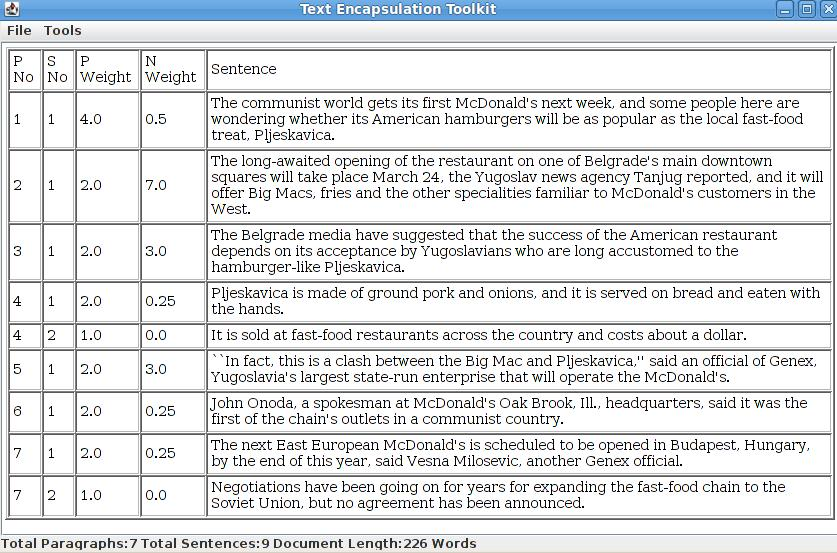
\includegraphics[width=0.9\textwidth]{/home/imran/Documents/myreport/Figure/pic1}
 \caption{\singlespace Text encapsulation toolkit identify important sentences, and phrases in text}
\end{figure}
\label{ch4:pnphrase}
After the source text is chunked in phrases, all noun chunks phrases are inspected with \emph{PosTagger} another class of \emph{OpenNLP tools API}
to determine proper noun phrases and their respective frequency through out the document. Part of speech tagger tags proper nouns as ``NNP''.
The weight based on proper noun phrases is computed as follows:
\begin{displaymath}
  weight\  based\ on\ proper\ nouns\  phrases = \frac{count\ of\ proper\ nouns in\ the\ sentence}
 {count\ of\ proper\ nouns\ in\ entire\ document}
\end{displaymath}
Sentences having zero weight based on proper noun phrases have very less probability to contribute to the extracts and are ignored. 

Extracts are generated by reading the sentences from the top of the document, ignoring sentences not containing any proper noun till the desired size of the summary(usually
one third of the size(number of words) of the source text) is reached. Since the test data comprises of news articles where important information frequently appear 
at the top of the document, sentences from the source text are sequentially added to extracts. It also helps in retaining coherence. Another argument to support the
procedure of extracts generation is that first segment (paragraph) of a text has been used as a base line method to evaluate auto generated summaries. If desired length
of extracts is not specified by the user, the extraction retains all sentences of the document except those having no proper nouns at all. Retaining the sentences in 
this way is also necessary if each sentence, included in the extract, should be encapsulated to represent corresponding paragraph. 

\begin{figure}[h]
 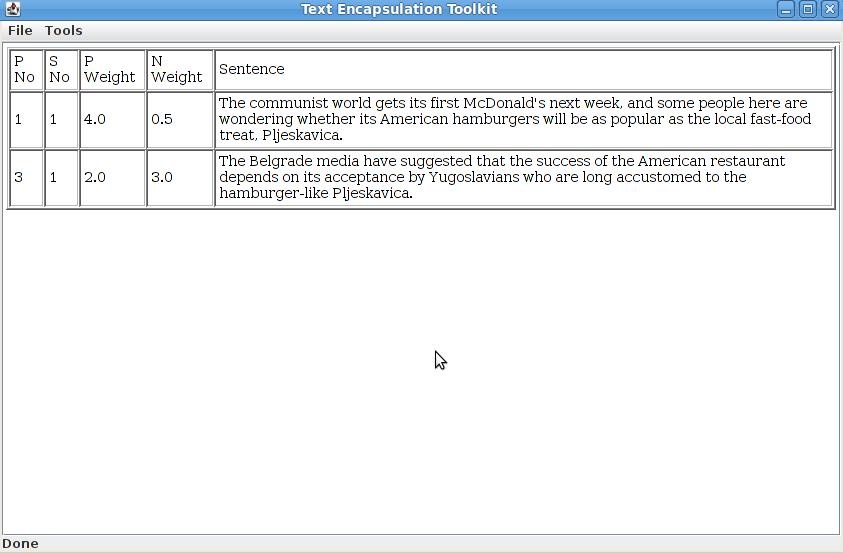
\includegraphics[width=0.9\textwidth]{/home/imran/Documents/myreport/Figure/pic2}
 \caption{\singlespace 70 words extracts obtained for the document shown in previous figure}
\end{figure}
\subsection{Encapsulation}
For each sentence present in extracts, a pattern of part of speech tags (i.e. noun phrase, verb phrase, noun phrase) is determined by iterating through the chunks 
generated using \emph{TreebankChunker}. The chunks are appended one after another in the order they occur in the sentence. Since the pattern only includes noun and verb
phrases discarding qualifying phrases such as \emph{ADVP}, adverb phrases etc., the encapsulation obtained may not be easily deciphered.

\begin{figure}[h]
 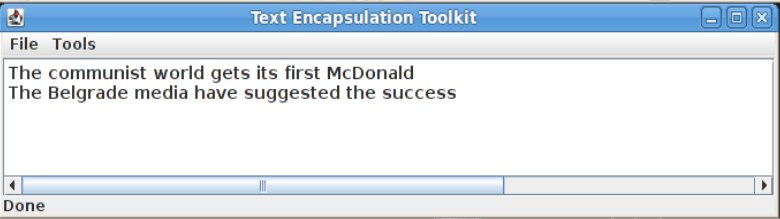
\includegraphics[width=0.9\textwidth]{/home/imran/Documents/myreport/Figure/pic3}
 \caption{\singlespace encapsulation obtained for the document shown in previous figure}
\end{figure}
